\documentclass[10pt,a4paper]{article}
\usepackage[utf8]{inputenc}
\usepackage[italian]{babel}
\usepackage{amsmath}
\usepackage{amsfonts}
\usepackage{amssymb}
\usepackage{graphicx}
\usepackage{gensymb}
\usepackage[left=2cm,right=2cm,top=2cm,bottom=2cm]{geometry}
\newcommand{\rem}[1]{[\emph{#1}]}

\author{Gruppo BN \\ Federico Belliardo, Marco Costa, Lisa Bedini}
\title{Lock in}
\begin{document}

\maketitle
\section{Scopo dell'esperienza}
Questa esperienza è finalizzata alla misura della costante di assorbimento del Mylar. Nella prima parte ci si propone di montare i circuiti e caratterizzarne il singolo funzionamento, successivamente procederemo a collegarli fra loro per eseguire la misura mediante lock-in.

%Si misurerà potenziale in funzione del numero di lastrine di Mylar\footnote{Resina termoplastica di indice di rifrazione pari a 1.5750 (utile?)} (e quindi ricavare il coefficiente di assorbimento di tale materiale) interposte fra la sorgente luminosa (LED) e il fotodiodo (fototransistor?). Infine verificheremo che il sistema non è sensibile alla luce ambientale\footnote{Una delle tante sorgenti di rumore.}%

\section{Materiale occorrente}
\begin{itemize}
\item TL082 (JFET input dual Op-Amp);
\item 4 TL081 (JFET input Op-Amp);
\item SN7400 (4 porte NAND);
\item DG441 (4 interruttori analogici CMOS);
\item 2N1711/BC182 (transistor NPN);
\item LED rosso;
\item fotodiodo;
\end{itemize}


Tutte le resistenze, i condensatori e la tensione di alimentazione sono stati misurati con il multimetro digitale, quindi l'errore è stato propagato secondo le specifiche nel manuale ($0.8% + 3 digit$ per le resistenze e $0.5 % + 1 digit$ per i voltaggi). I tempi e le restanti tensioni sono state misurate con i cursori dell'oscilloscopio: l'errore sui tempi è dato dalla risoluzione dei cursori stessi mentre quello sulle tensioni è stato propagato considerando sia l'errore sul posizionamento dei cursori sia l'errore sistematico del $3\%$.

\section{Schema a blocchi}
Il circuito Lock-in è usato per effettuare misure di segnali deboli in un ambiente molto rumoroso. Nel nostro caso il segnale è la luce emessa dal LED. Tale segnale non è continuo ma modulato da un' onda sinusoidale prodotta dal generatore di funzioni. Abbiamo scelto una frequenza pari a $1\,\mbox{kHz}$ per eliminare il rumore \emph{1/f} dovuto alla presenza di dispositivi attivi\footnote{Può essere prodotto dalle discontinuità intrinseche dei materiali costruttivi.}. In figura \ref{fig:schemablocchi} si nota come questo circuito complesso sia costituito da sottocircuiti (che saranno analizzati e spiegati successivamente); in particolare nella parte superiore dello schema si trovano i circuiti che servono a sfruttare sia la parte positiva che negativa del segnale per la misura e nella parte inferiore si trovano i circuiti di amplificazione del segnale da misurare.

\begin{figure}[!htb]
  \centering
  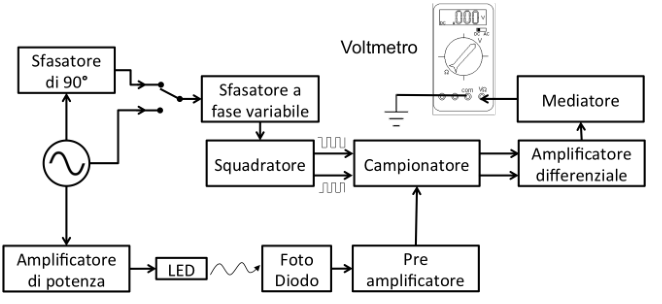
\includegraphics[scale=0.75]{schemablocchi.png}
\caption{Schema a blocchi del circuito Lock-in.\label{fig:schemablocchi}}
\end{figure}
\\

\section{Implementazione schema a blocchi}

\subparagraph{Amplificatore di potenza e preamplificatore}
Abbiamo montato il circuito in figura \ref{fig:ampli-preampli} misurando tramite multimetro digitale: $R_1=10k$, $R_2=1.5k$, $R_3=82k$, $R_4=56k$, $R_5=18k$, $R_6=120k$, $R_7=3.9k$, $R_9=1.2M$, $C_1=100n$ e $C_2=100n$.\\

Il circuito consiste in un amplificatore di potenza realizzato con un transistor npn che permette di pilotare l'accessione del Led con l'onda del generatore di funzioni, che controlla la corrente in base.
Il transistor è dotato di circuito di polarizzazione quindi come anticipato prima l'effetto del segnale alternato è di modulare la corrente di collettore e quindi l'intensità luminosa.
Nella seconda parte (elettricamente separata dalla prima) troviamo un  circuito di lettura del fotodiodo, che grazie all'opAmp presenta un alta impedenza di ingresso e bassa impedenza di uscita e permette quindi di osservare la risposta del diodo senza alterarla.
Il segnale del fotodiodo viene poi derivato (per ottenere un segnale a media nulla) e mandato in un comune amplificatore non invertente.\\

\subparagraph{Misura della costante di assorbimento senza Lock-in}
Per limitare l'influenza della luce ambientale tutte le seguenti misure sono state eseguite coprendo l'apparato con %TODO %che cosa?%.
Si è inviato all'ingresso (S1) un segnale sinusoidale di frequenza pari a $1\pm  kHz$ e ampiezza picco-picco $V_{pp}= 6 \pm \,\mbox{V}$. All'uscita (S6) si ottiene la forma d'onda sinusoidale in figura \ref{fig:S6} che ha ampiezza TOT. Abbiamo ripetuto la misura della tensione in uscita in funzione del numero $n$ di lastrine di Mylar poste fra LED e fotodiodo, i dati sono rappresentati in tabella \ref{tab:ampli-preampli}. Sapendo che l'andamento teorico della tensione è $V_{out}=V_0exp(-n/n_0)$ si è fatto il grafico e eseguito il fit, ottenendo n_0= V_0= chi^2=. Conoscendo lo spessore costante delle lastrine ($150\mu \mbox{m}$) si osserva che il numero $n$ è direttamente proporzionale alla lunghezza percorsa dalla luce nel Mylar. Sostituendo otteniamo direttamente a esponente della legge la lunghezza caratteristica di assorbimento: x_0= TOT.

\begin{figure}[!htb]
  \centering
  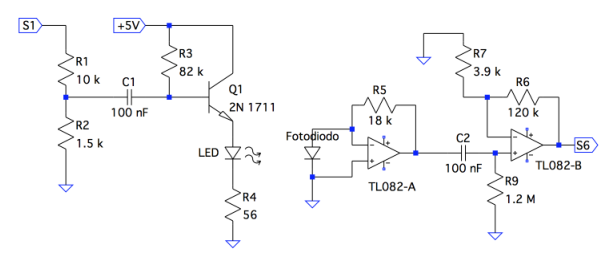
\includegraphics[scale=0.75]{ampli-preampli.png}
\caption{Schema a blocchi del circuito Lock-in.\label{fig:ampli-preampli}}
\end{figure}

IMMAGINI OSCILLOSCOPIO USCITA E RUMORE PER STIMA
TABELLA DATI
GRAFICO E FIT VvsNUMERO LASTRINE
SENSIBILE A LUCE AMBIENTALE?
%Dire eventualemnte se si osserva rumore alla frequenza delle lampade, che è 50 Hz$

\subparagraph{Sfasatore di 90\degree e sfasatore variabile}
I circuiti relativi sono quelli in figura \ref{fig:sfasatori}. L'ingresso S1 è ancora riferito all'uscita del generatore di funzioni. Abbiamo regolato il trimmer P1 in modo da ottenere in S2 la stessa forma d'onda dell'ingresso sfasata di 90\degree (figura \ref{osc:sfasatore90}). In S3 l'uscita sarà un'onda quadra e abbiamo regolato il trimmer P3 in modo che il \emph{duty cycle} fosse pari al 50\% (ciò è stato verificato con l'opportuna funzione dell'oscilloscopio). Se si agisce sul deviatore si bypassa lo sfasatore quindi all'ingresso dello sfasatore variabile l'onda sarà la stesa in ingresso a S1.\\
L'analisi dello sfasatore mostra che esso ha una funzione di trasferimento nel dominio di Laplace: $G(s) = \frac{1-s(R_{16} +P_1) C_{4}}{1+s(R_{16} + P_1)C_{4}}$ dunque si tratta di una fase che può essere scelta calibrando il trimmer $P_1$.\\
%TODO Spiegare perchè si può cambiare il duty cycle.


LIMITI TRIMMER P2 PER REGOLARE SFASAMENTO
IMMAGINI CON E SENZA DEVIATORE
IMMAGINI ONDE ALLE USCITE

\begin{figure}[!htb]
  \centering
  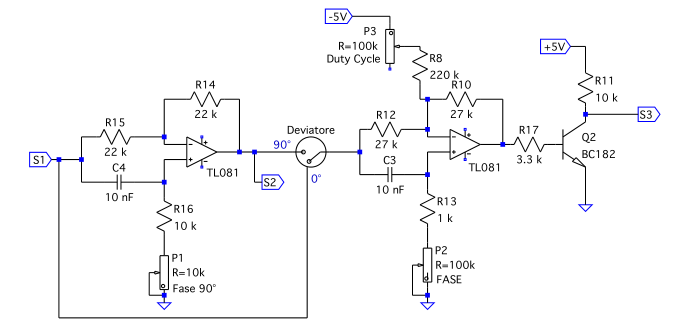
\includegraphics[scale=0.75]{sfasatori.png}
\caption{Schema circuitale dello sfasatore di 90\degree e dello sfasatore variabile.\label{fig:sfasatori}}
\end{figure}


\subparagraph{Squadratore e campionatore}
Abbiamo montato i circuiti in figura \ref{fig:sqadratore-campionatore}. Ricordiamo che S3 corrisponde all'onda quadra in uscita dallo sfasatore variabile e viene inviato ai due NOT U1 e U2 (che hanno la funzione di ripulire il segnale), quindi il segnale S4 e il suo negato S5 vengono mandati al campionatore che ha la funzione di alternare il canale in cui deve andare l'onda S6.

IMMAGINI DELLE ONDE
S4 e S5 IN OPPOSIZIONE DI FASE
S7 E S8 NELLE CONFIGURAZIONI DEL DEVIATORE

\begin{figure}[!htb]
  \centering
  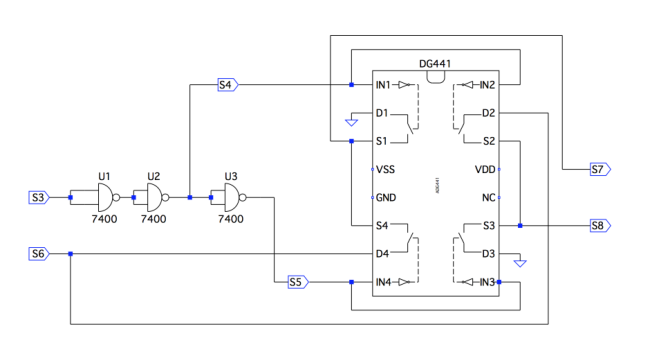
\includegraphics[scale=0.75]{sqadratore-campionatore.png}
\caption{Schema circuitale dello squadratore e del campionatore.\label{fig:sqadratore-campionatore}}
\end{figure}


\subparagraph{Amplificatore differenziale e mediatore}
Infine abbiamo realizzato il circuito in figura \ref{fig:amplificatorediff-mediatore}. Le onde agli ingressi S7 e S8 (invertito) sono sommate dall'amplificatore differenziale, la cui uscita è resa continua dal mediatore (filtro passa-basso)

IMMAGINI DI TUTTE LE ONDE CON DEVIATORE 0/90
ONDA S9 PER POSIZIONI DEVIATORE%ci si aspetta sempre stesso segno/segnale a media nulla
VOLTMETRO DEVE DARE MEDIA DEL SEGNALE IN INGRESSO
IMMAGINE TENSIONE CONTINUA
REGOLARE FASE P2 T.C. CON 90° VOLTMETRO=0 %compensazione fasi
NELLA POSIZIONE 0° TENSIONE ESPONENZIALE

\begin{figure}[!htb]
  \centering
  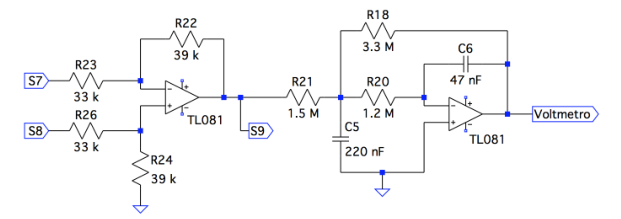
\includegraphics[scale=0.75]{amplificatorediff-mediatore.png}
\caption{Schema a blocchi del circuito Lock-in.\label{fig:amplificatorediff-mediatore}}
\end{figure}

\\
\section{Presa dati}

TABELLA DATI
IMMAGINE E FIT


\\

\section{Conclusioni}

CONFRONTO DEI VALORI OTTENUTI CON E SENZA LOCK-IN E COMMENTI

\\
\begin{table}[!htb]
\centering
\begin{tabular}{|c|c|c|c|}
\hline 
$R_i [\Omega ]$ & $\Delta R_i [\Omega ]$ & $t [\mu s]$ & $\Delta t [\mu s]$\\
\hline
 327 &  3 & 25.8 & 0.2\\ 
\hline 
 470 &  4 & 41.6 & 0.2\\ 
\hline
 669 &  5 & 69.2 & 0.6\\ 
\hline
 824 &  7 & 82 & 1\\ 
\hline 
 984 &  8 & 102 & 1\\ 
\hline
 1183 &  9 & 118 & 1\\ 
\hline
 1454 &  11 & 140 & 1\\ 
\hline
\end{tabular} 
\caption{Presa dati per verificare la linearità fra $R$ e $t$.\label{tab:monostabile}}
\end{table}


\end{document}